% !TeX root = ..\studio-operation-guide.tex
\section{Call Hold/Resume}

You can place an active call on hold. Only one active call can be in
progress at any time. Other calls can be made and received while placing
the original call on hold. When you place a call on hold, your IP PBX
may play music to the other party while waiting.

\subsubsection{To place a call on hold:}

\begin{enumerate}
	\item Press	\scalerel*{
\includegraphics{images/yealink/btn-hold.png}}{B}
		or the \textbf{Hold} soft key during a call.
	
		The LCD screen indicates that the call is on hold and the line key LED
		flashes green.
	
		\begin{figure}[h]
			\centering
			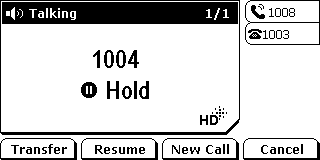
\includegraphics{images/yealink/screen-006.png}
		\end{figure}
\end{enumerate}

\begin{quote}
	\textbf{Note}
	
	The phone will beep softly every 30 seconds to remind you that you still
	have a call on hold.
\end{quote}

\subsubsection{To resume a held call:}

\begin{enumerate}
	\item Press \scalerel*{
\includegraphics{images/yealink/btn-hold.png}}{B}
		or the \textbf{Resume} soft key.
\end{enumerate}

\subsubsection{Multiple Calls on Hold:}

If multiple calls are placed on hold, do one of the following:

\begin{itemize}
	\item Press \scalerel*{
\includegraphics{images/yealink/btn-up.png}}{B} or
		\scalerel*{
\includegraphics{images/yealink/btn-down.png}}{B} to switch
		between the calls, and then press the \textbf{Resume} soft key to
		retrieve the desired call.
	\item Press the corresponding line key to retrieve the desired call.
\end{itemize}

A numbered prompt appears on the LCD screen, for example "2/4",
indicating that this is the second call out of four calls.
